% Options for packages loaded elsewhere
% Options for packages loaded elsewhere
\PassOptionsToPackage{unicode}{hyperref}
\PassOptionsToPackage{hyphens}{url}
\PassOptionsToPackage{dvipsnames,svgnames,x11names}{xcolor}
%
\documentclass[
  british,
  a4paper,
]{article}
\usepackage{xcolor}
\usepackage{amsmath,amssymb}
\setcounter{secnumdepth}{-\maxdimen} % remove section numbering
\usepackage{iftex}
\ifPDFTeX
  \usepackage[T1]{fontenc}
  \usepackage[utf8]{inputenc}
  \usepackage{textcomp} % provide euro and other symbols
\else % if luatex or xetex
  \usepackage{unicode-math} % this also loads fontspec
  \defaultfontfeatures{Scale=MatchLowercase}
  \defaultfontfeatures[\rmfamily]{Ligatures=TeX,Scale=1}
\fi
\usepackage{lmodern}
\ifPDFTeX\else
  % xetex/luatex font selection
\fi
% Use upquote if available, for straight quotes in verbatim environments
\IfFileExists{upquote.sty}{\usepackage{upquote}}{}
\IfFileExists{microtype.sty}{% use microtype if available
  \usepackage[]{microtype}
  \UseMicrotypeSet[protrusion]{basicmath} % disable protrusion for tt fonts
}{}
\makeatletter
\@ifundefined{KOMAClassName}{% if non-KOMA class
  \IfFileExists{parskip.sty}{%
    \usepackage{parskip}
  }{% else
    \setlength{\parindent}{0pt}
    \setlength{\parskip}{6pt plus 2pt minus 1pt}}
}{% if KOMA class
  \KOMAoptions{parskip=half}}
\makeatother
% Make \paragraph and \subparagraph free-standing
\makeatletter
\ifx\paragraph\undefined\else
  \let\oldparagraph\paragraph
  \renewcommand{\paragraph}{
    \@ifstar
      \xxxParagraphStar
      \xxxParagraphNoStar
  }
  \newcommand{\xxxParagraphStar}[1]{\oldparagraph*{#1}\mbox{}}
  \newcommand{\xxxParagraphNoStar}[1]{\oldparagraph{#1}\mbox{}}
\fi
\ifx\subparagraph\undefined\else
  \let\oldsubparagraph\subparagraph
  \renewcommand{\subparagraph}{
    \@ifstar
      \xxxSubParagraphStar
      \xxxSubParagraphNoStar
  }
  \newcommand{\xxxSubParagraphStar}[1]{\oldsubparagraph*{#1}\mbox{}}
  \newcommand{\xxxSubParagraphNoStar}[1]{\oldsubparagraph{#1}\mbox{}}
\fi
\makeatother


\usepackage{longtable,booktabs,array}
\newcounter{none} % for unnumbered tables
\usepackage{calc} % for calculating minipage widths
% Correct order of tables after \paragraph or \subparagraph
\usepackage{etoolbox}
\makeatletter
\patchcmd\longtable{\par}{\if@noskipsec\mbox{}\fi\par}{}{}
\makeatother
% Allow footnotes in longtable head/foot
\IfFileExists{footnotehyper.sty}{\usepackage{footnotehyper}}{\usepackage{footnote}}
\makesavenoteenv{longtable}
\usepackage{graphicx}
\makeatletter
\newsavebox\pandoc@box
\newcommand*\pandocbounded[1]{% scales image to fit in text height/width
  \sbox\pandoc@box{#1}%
  \Gscale@div\@tempa{\textheight}{\dimexpr\ht\pandoc@box+\dp\pandoc@box\relax}%
  \Gscale@div\@tempb{\linewidth}{\wd\pandoc@box}%
  \ifdim\@tempb\p@<\@tempa\p@\let\@tempa\@tempb\fi% select the smaller of both
  \ifdim\@tempa\p@<\p@\scalebox{\@tempa}{\usebox\pandoc@box}%
  \else\usebox{\pandoc@box}%
  \fi%
}
% Set default figure placement to htbp
\def\fps@figure{htbp}
\makeatother



\ifLuaTeX
\usepackage[bidi=basic,shorthands=off]{babel}
\else
\usepackage[bidi=default,shorthands=off]{babel}
\fi
\ifLuaTeX
  \usepackage{selnolig} % disable illegal ligatures
\fi


\setlength{\emergencystretch}{3em} % prevent overfull lines

\providecommand{\tightlist}{%
  \setlength{\itemsep}{0pt}\setlength{\parskip}{0pt}}



 


\makeatletter
\@ifpackageloaded{tcolorbox}{}{\usepackage[skins,breakable]{tcolorbox}}
\@ifpackageloaded{fontawesome5}{}{\usepackage{fontawesome5}}
\definecolor{quarto-callout-color}{HTML}{909090}
\definecolor{quarto-callout-note-color}{HTML}{0758E5}
\definecolor{quarto-callout-important-color}{HTML}{CC1914}
\definecolor{quarto-callout-warning-color}{HTML}{EB9113}
\definecolor{quarto-callout-tip-color}{HTML}{00A047}
\definecolor{quarto-callout-caution-color}{HTML}{FC5300}
\definecolor{quarto-callout-color-frame}{HTML}{acacac}
\definecolor{quarto-callout-note-color-frame}{HTML}{4582ec}
\definecolor{quarto-callout-important-color-frame}{HTML}{d9534f}
\definecolor{quarto-callout-warning-color-frame}{HTML}{f0ad4e}
\definecolor{quarto-callout-tip-color-frame}{HTML}{02b875}
\definecolor{quarto-callout-caution-color-frame}{HTML}{fd7e14}
\makeatother
\makeatletter
\@ifpackageloaded{caption}{}{\usepackage{caption}}
\AtBeginDocument{%
\ifdefined\contentsname
  \renewcommand*\contentsname{Table of contents}
\else
  \newcommand\contentsname{Table of contents}
\fi
\ifdefined\listfigurename
  \renewcommand*\listfigurename{List of Figures}
\else
  \newcommand\listfigurename{List of Figures}
\fi
\ifdefined\listtablename
  \renewcommand*\listtablename{List of Tables}
\else
  \newcommand\listtablename{List of Tables}
\fi
\ifdefined\figurename
  \renewcommand*\figurename{Figure}
\else
  \newcommand\figurename{Figure}
\fi
\ifdefined\tablename
  \renewcommand*\tablename{Table}
\else
  \newcommand\tablename{Table}
\fi
}
\@ifpackageloaded{float}{}{\usepackage{float}}
\floatstyle{ruled}
\@ifundefined{c@chapter}{\newfloat{codelisting}{h}{lop}}{\newfloat{codelisting}{h}{lop}[chapter]}
\floatname{codelisting}{Listing}
\newcommand*\listoflistings{\listof{codelisting}{List of Listings}}
\makeatother
\makeatletter
\makeatother
\makeatletter
\@ifpackageloaded{caption}{}{\usepackage{caption}}
\@ifpackageloaded{subcaption}{}{\usepackage{subcaption}}
\makeatother
\usepackage{bookmark}
\IfFileExists{xurl.sty}{\usepackage{xurl}}{} % add URL line breaks if available
\urlstyle{same}
% fallback for those not using the hyperref driver hyperxmp:
\makeatletter
\@ifundefined{xmpquote}{\newcommand{\xmpquote}[1]{#1}}{}
\makeatother
\hypersetup{
  pdftitle={An AI-assisted workflow for macroeconomic models},
  pdfauthor={Carlos Galindo},
  pdflang={en-GB},
  colorlinks=true,
  linkcolor={blue},
  filecolor={Maroon},
  citecolor={Blue},
  urlcolor={Blue},
  pdfcreator={LaTeX via pandoc}}


\title{An AI-assisted workflow for macroeconomic models}
\usepackage{etoolbox}
\makeatletter
\providecommand{\subtitle}[1]{% add subtitle to \maketitle
  \apptocmd{\@title}{\par {\large #1 \par}}{}{}
}
\makeatother
\subtitle{Evidence sourced in tiers, dated and logged, and
machine-written code audited by tests, so every output can be checked}
\author{Carlos Galindo}
\date{}
\begin{document}
\maketitle


\begin{tcolorbox}[enhanced jigsaw, arc=.35mm, bottomrule=.15mm, breakable, colback=white, colframe=quarto-callout-note-color-frame, left=2mm, leftrule=.75mm, opacityback=0, rightrule=.15mm, toprule=.15mm]

\vspace{-3mm}\textbf{At a glance}\vspace{3mm}

\begin{itemize}
\tightlist
\item
  \textbf{Question.} If an AI assistant writes much of the code and
  drafts much of the analysis, what makes the output safe to rely on?
\item
  \textbf{Approach.} Wrap a small macroeconomic model in a research
  protocol: sources are ranked in tiers, every figure is dated, every
  transformation is logged, and every piece of machine-written code must
  pass tests before its output counts.
\item
  \textbf{Finding.} The pieces fit together into a workflow that ran end
  to end on simulated data, with a provenance record and an audit trail
  for each run, and with its own gaps stated openly.
\item
  \textbf{Why it matters.} Speed from AI assistance is only useful in
  economics if the result stays checkable. Here the checking is part of
  the design, not an afterthought.
\end{itemize}

\end{tcolorbox}

\subsection{The question}\label{the-question}

Macroeconomic work now leans on assistants that can draft a model, fetch
a number and write the code that estimates it in minutes. The risk is
not that they are slow. It is that they are fluent: a wrong number, a
stale release or a silently changed transformation reads exactly like a
right one. A reader who sees only the final table cannot tell which
numbers were observed, which were proxied, how old they were, or whether
the code that produced them did what it was meant to do.

The obvious response, reviewing the output by eye, does not scale and
does not catch the errors that matter, because the reviewer sees the
same polished surface the author does. The question this project
addresses is therefore practical: how do you build a research workflow
in which an AI assistant does a great deal of the work, yet each output
can be traced to its sources, dated, and tested, so that a sceptical
reader can re-check it?

The setting was a family of small macroeconomic models for open
economies, begun as a set of equations and a research protocol and then
turned into a tested implementation during 2025. The models combine a
standard New Keynesian block (an output gap, a Phillips curve and a
policy rule) with political-credibility and capital-flow terms that
enter through the exchange-rate and risk-premium channels. The workflow
around them is the subject here, not the models' forecasts.

\subsection{Approach}\label{approach}

The workflow has three layers, each answering a different way the output
could go wrong.

\subsubsection{Sources in tiers, dated}\label{sources-in-tiers-dated}

The first layer is a protocol that the assistant must follow whenever it
gathers evidence. Sources are ranked in four tiers, from authoritative
official statistics down to supplementary and proxy series. Official
sources come first; where they are stale, a newer but less authoritative
series may be added alongside them, with its credibility noted, and the
official figure is retained rather than overwritten. When two sources
disagree, a fixed order decides which is reported and the disagreement
is flagged.

Every figure carries its source and its date. An authoritative release
more than one month old is explicitly marked as outdated in the text.
That small rule does a lot of work: it turns a vague worry about
timeliness into something a reader sees on the page. Where a variable
cannot be observed in time, the protocol requires a higher-frequency
proxy with a stated rationale, for example a monthly activity indicator
standing in for quarterly output, and the proxy is labelled as such.

\subsubsection{Transformations logged for
provenance}\label{transformations-logged-for-provenance}

The second layer is a record. Every raw file is stored with a content
fingerprint and the date it was fetched. Every transformation applied to
it, such as annual differences, trend-gap calculations and
normalisation, is written to a provenance log, so that a later reader
can see not just what a number is but how it came to be. Parameters,
matrix dimensions and the mapping from observed series to model states
are written to an inventory alongside each run, and a generated report
places the measured series next to the model's reconstruction of them,
with the state taxonomy and diagnostics laid out for review.

\subsubsection{Machine-written code audited by
tests}\label{machine-written-code-audited-by-tests}

The third layer addresses the code itself. The implementation is a
linear state-space model estimated with a Kalman filter, a smoother and
an expectation-maximisation routine, extended to handle mixed
frequencies: a monthly state is measured partly through quarterly
observations. The political and capital-flow terms are mapped from
underlying indicators into model shocks through a deliberately
conservative mapping. The code was largely written with AI assistance,
and the progress documents are themselves agent-maintained. That is
precisely why it is wrapped in tests. Component-level tests check
individual pieces; equivalence tests check that an optional extension,
when switched off, reproduces the baseline exactly; stability tests
check that estimation behaves across a grid of settings; and an
end-to-end test generates simulated data, runs the whole cycle and
confirms that the expected artefacts exist and have the right shapes. A
verification step fails the run if any of them is missing.

All of this was exercised end to end on simulated data. That choice is
deliberate and is part of the claim: the aim was to prove the workflow,
not to publish estimates.

\subsection{What the work shows}\label{what-the-work-shows}

The first result is structural. The three layers compose: a figure in a
report can be followed back through its transformations to a dated,
tiered source, and the code that produced it has passed checks that do
not depend on anyone's recollection of what it was supposed to do. The
workflow is a method for making AI-produced economics inspectable, and
it was shown to run end to end.

The second result is about what the tests can and cannot see. Simulated
data allow a check that real data never do: the true state is known, so
the filter's reconstruction can be compared with it. The first figure
shows the shape of that check for a mixed-frequency setting, where the
latent monthly state is observed only every third month. The band is
narrow in the months with a fresh observation and widens in between,
which is the behaviour the audit should confirm.

\begin{figure}

\centering{

\pandocbounded{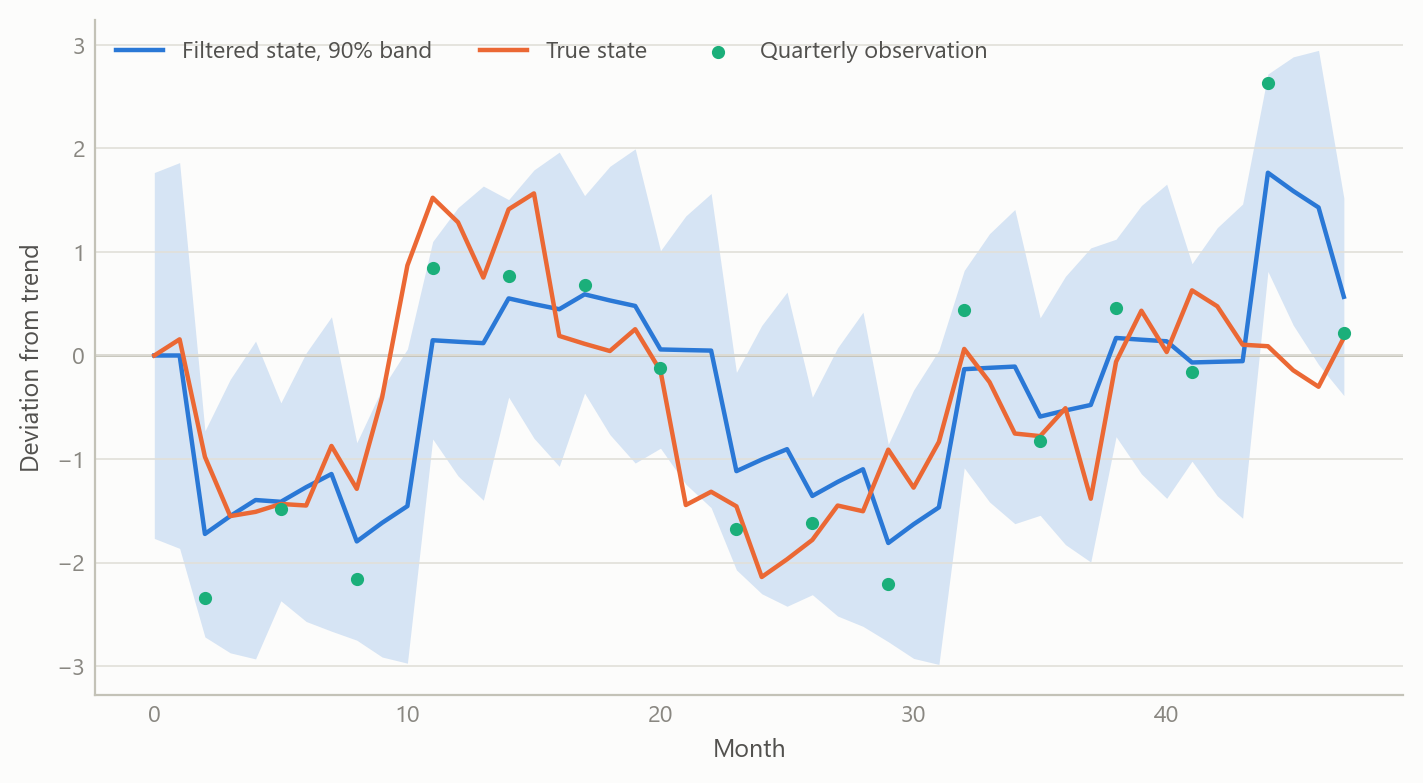
\includegraphics[keepaspectratio]{index_files/figure-latex/fig-state-output-1.png}}

}

\caption{\label{fig-state}A latent monthly state recovered by a filter
when only every third month is observed, against the known truth
(simulated data).}

\end{figure}%

The third result concerns the sourcing rules. The second figure shows
what the dating rule does to a simulated evidence set: items are drawn
from four tiers with different release lags, and those older than one
month are flagged. The point is not the particular ages but that the
flagged share is visible, per tier, before anyone reads the analysis.

\begin{figure}

\centering{

\pandocbounded{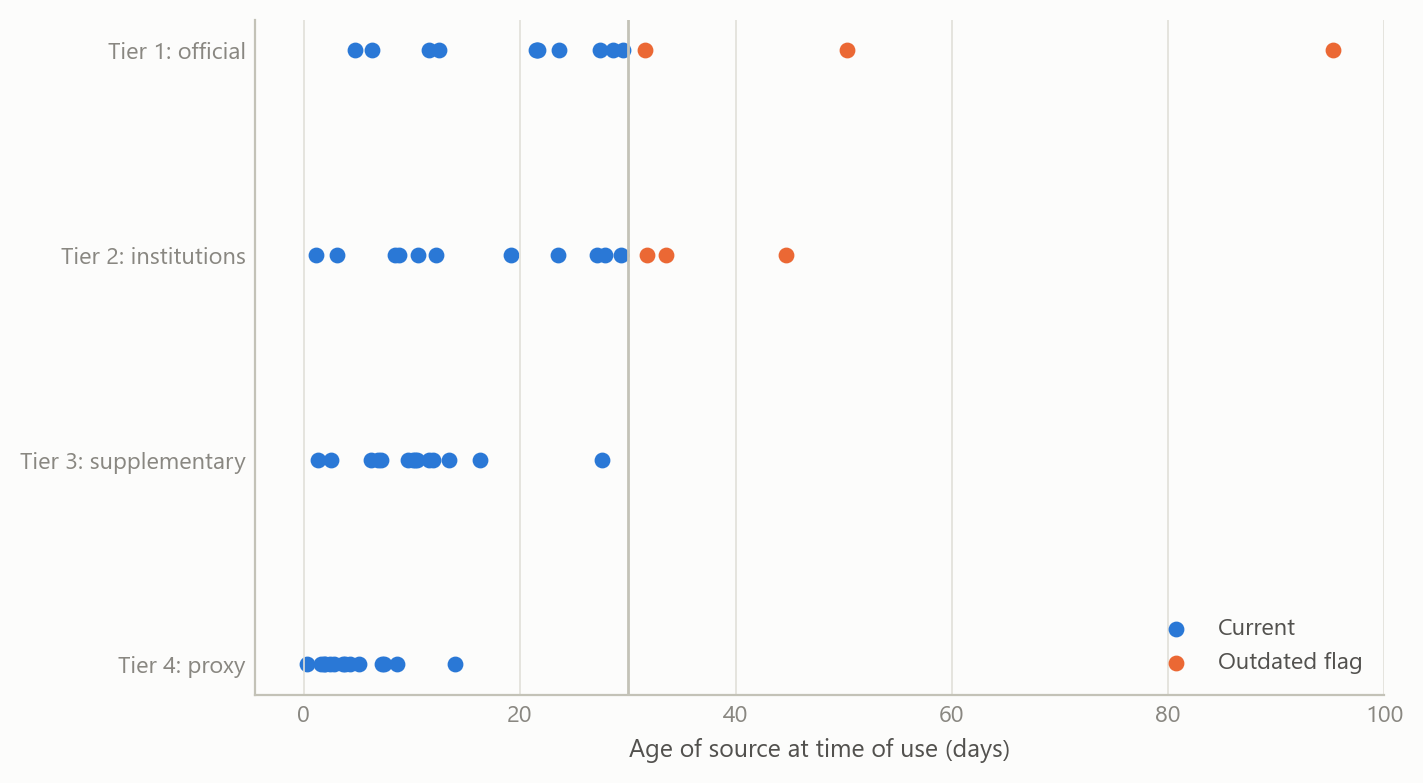
\includegraphics[keepaspectratio]{index_files/figure-latex/fig-tiers-output-1.png}}

}

\caption{\label{fig-tiers}Age of simulated evidence items by source
tier; items older than one month are flagged as outdated (simulated
data).}

\end{figure}%

The fourth result is the equivalence audit. The political-risk
correction is optional and additive. The test is that with its weight at
zero the corrected run must reproduce the baseline exactly, and that the
difference must grow smoothly as the weight rises. The third figure
shows that check on a simulated forecast. A failure at zero would reveal
a coding error that no amount of reading the output would catch.

\begin{figure}

\centering{

\pandocbounded{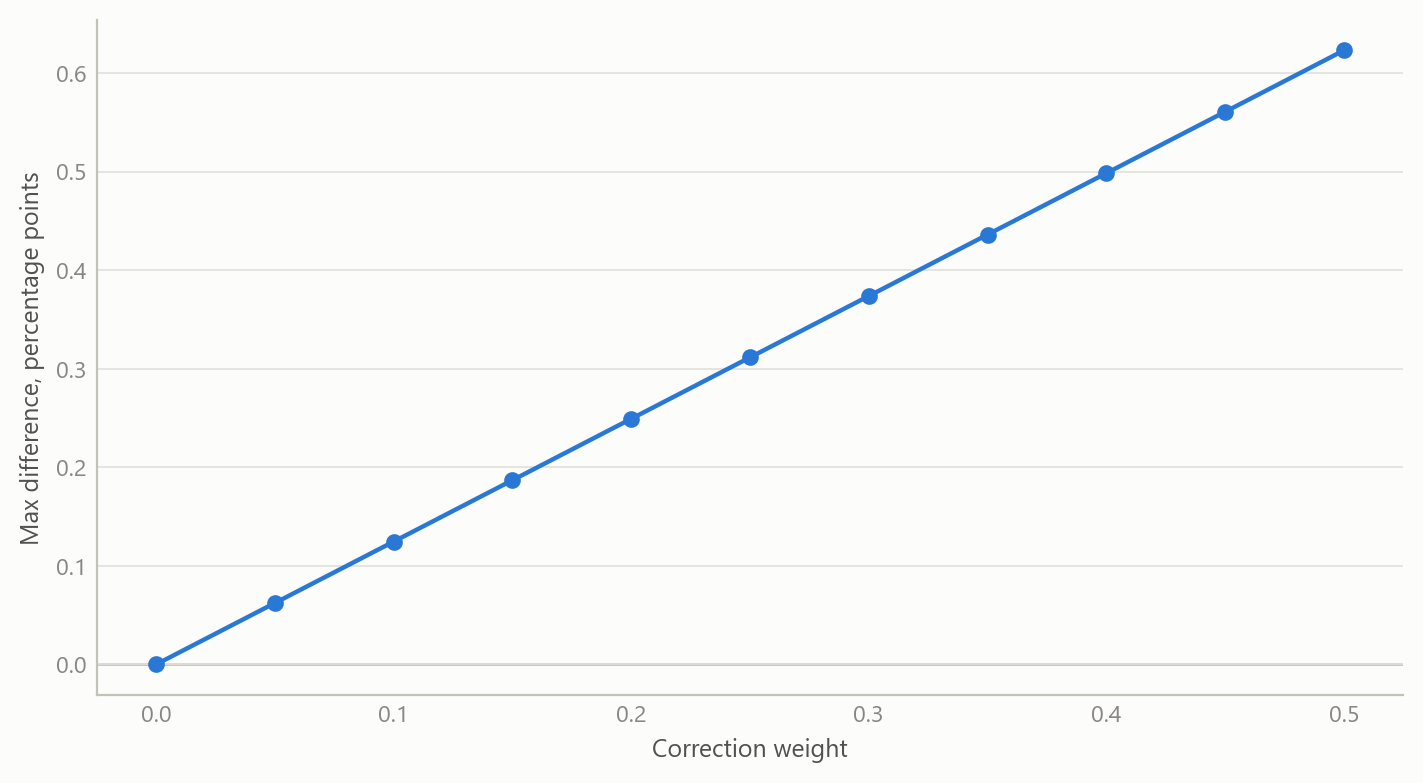
\includegraphics[keepaspectratio]{index_files/figure-latex/fig-equiv-output-1.png}}

}

\caption{\label{fig-equiv}Largest forecast difference between a run with
the optional correction and the baseline run, by correction weight
(simulated data).}

\end{figure}%

\subsection{Insights}\label{insights}

\begin{itemize}
\tightlist
\item
  \textbf{Fluency is the hazard, so provenance has to be mechanical.} A
  rule such as ``flag anything older than one month'' is cheap,
  objective and visible. Reviewing for quality by eye is none of those.
\item
  \textbf{Tests are the assistant's supervisor.} When code is
  machine-written, the tests carry the authority. A component that
  passes equivalence and stability checks is trusted for what it was
  tested to do, and no more.
\item
  \textbf{Simulated data are the right first proof.} Known truth makes
  it possible to verify that a pipeline recovers what it should, and it
  removes any temptation to read results into an unfinished system.
\item
  \textbf{Keep optional extensions optional.} Building additions as
  switchable, additive layers with an exact-equivalence test at the off
  position made it safe to extend the baseline model without losing the
  ability to verify it.
\item
  \textbf{Write the gaps down.} The project's own assurance summary
  lists what is missing. Naming the gaps is part of what makes the rest
  credible.
\end{itemize}

\subsection{Scope and next steps}\label{scope-and-next-steps}

The workflow is built to make machine-assisted model building traceable
end to end: each number carries its source, its age and the code that
produced it, and the model's filter is checked on simulated data, where
the true state is known.

The natural extensions are three. First, solving the full
forward-looking model with rational expectations, a complete fiscal debt
block and the political-risk adjustment inside the policy rule, and
confirming that it reduces to the current core in the appropriate limit.
Second, running the same logged workflow on real data and comparing its
audit trail with the simulated one. Third, turning the checks into an
automated gate that stops any run whose expected outputs or provenance
records are missing.

The full protocol and worked examples can be discussed on request.

\subsection{About the evidence}\label{about-the-evidence}

The work was carried out during 2025 as part of a rebuild of
macroeconomic modelling capability. It rests on a written research
protocol, a tested implementation and generated audit reports, all
exercised on simulated data; no real-data estimates are claimed. The
figures above are simulated and show the logic of each check, not the
project's results.

Figures and tables marked \emph{simulated} are generated from simulated
data built to share the structure of the analysis (its variables,
horizons and frequencies). They show how each method works and what its
output looks like. Results stated in the text, and figures that give a
source, are the project's own. Methods are described at the level of a
methods section. Code and data pipelines are not reproduced here.




\end{document}
